\documentclass[
  12pt,
  openright,
  oneside,
  a4paper,
  brazilian
]{abntex2}

\usepackage[T1]{fontenc}
\usepackage[utf8]{inputenc}
\usepackage{newtxtext,newtxmath}
\usepackage{indentfirst}
\usepackage{graphicx}
\usepackage{booktabs}
\usepackage{amsmath}
\usepackage{float}
\usepackage{microtype}
\usepackage{caption}
\usepackage{subcaption}
\usepackage{chngcntr}
\usepackage{setspace}
\usepackage{geometry}
\usepackage{fancyhdr}
\usepackage[alf]{abntex2cite}

\geometry{
  a4paper,
  top=3cm,
  left=3cm,
  bottom=2cm,
  right=2cm
}

\setlength{\parindent}{1.25cm}
\setlength{\parskip}{0pt}
\OnehalfSpacing

\pagestyle{fancy}
\fancyhf{}
\fancyhead[R]{\thepage}
\renewcommand{\headrulewidth}{0pt}

\DeclareCaptionFont{eventten}{\fontsize{10}{12}\selectfont}
\DeclareCaptionLabelFormat{eventhyphen}{#1~#2 -}

\captionsetup{
  justification=centering,
  font=eventten
}

\captionsetup[figure]{
  name=Figura,
  labelformat=eventhyphen,
  labelsep=none,
  labelfont=normalfont,
  textfont=normalfont,
  font=eventten,
  position=above
}

\captionsetup[table]{
  name=Tabela,
  labelformat=eventhyphen,
  labelsep=none,
  labelfont=normalfont,
  textfont=normalfont,
  font=eventten
}

\counterwithout{section}{chapter}
\setcounter{section}{0}
\setcounter{subsection}{0}
\renewcommand{\thesection}{\arabic{section}}
\renewcommand{\thesubsection}{\thesection.\arabic{subsection}}

\newcommand{\eventsection}[1]{%
  \refstepcounter{section}%
  \setcounter{subsection}{0}%
  \par\addvspace{1.2\baselineskip}%
  \noindent\textbf{\thesection.\ \MakeUppercase{#1}}\par
  \nobreak\vspace{0.7\baselineskip}%
}

\newcommand{\eventsubsection}[1]{%
  \refstepcounter{subsection}%
  \par\addvspace{\baselineskip}%
  \noindent\textbf{\thesubsection\ #1}\par
  \nobreak\vspace{0.5\baselineskip}%
}

\newcommand{\artigofonte}[1]{
  \vspace{0.2cm}
  \begin{center}
    \fontsize{10}{12}\selectfont Fonte: #1
  \end{center}
}

\newcommand{\tabelafonte}{\fontsize{10}{12}\selectfont}
\renewcommand{\bibname}{REFER\^ENCIAS}
\renewcommand{\bibsection}{%
  \par\addvspace{1.2\baselineskip}%
  \noindent\textbf{\MakeUppercase{\bibname}}\par
  \nobreak\vspace{0.7\baselineskip}%
}

\titulo{AVALIA\c{C}\~AO COMPARATIVA DE ALGORITMOS DE BOOSTING E BAGGING PARA DETEC\c{C}\~AO DE SURTOS DE MAL\'ARIA NO ESTADO DO AMAZONAS, BRASIL}
\autor{Nome do(a) Autor(a) 1\thanks{Institui\c{c}\~ao, e-mail.} \and Nome do(a) Autor(a) 2\thanks{Institui\c{c}\~ao, e-mail.}}
\data{2026}

\begin{document}

\begin{center}
{\bfseries\MakeUppercase{\thetitle}}
\end{center}

\begin{center}
\textit{Submiss\~ao sem identifica\c{c}\~ao de autoria}
\end{center}

\begin{center}
\textit{Os dados de autoria, institui\c{c}\~ao e e-mail ser\~ao informados ap\'os a avalia\c{c}\~ao.}
\end{center}

\begin{center}
\textbf{Eixo tem\'atico:} Ci\^encias, Tecnologias e Sa\'ude na Amaz\^onia
\end{center}

\noindent\textbf{Resumo}

\vspace{0.3cm}
\noindent
Este artigo apresenta uma avalia\c{c}\~ao comparativa entre algoritmos de \textit{bagging} e \textit{boosting} para detec\c{c}\~ao de surtos de mal\'aria no estado do Amazonas. O estudo utiliza dados municipais com vari\'aveis epidemiol\'ogicas e clim\'aticas, al\'em de atributos temporais derivados, para construir um pipeline de predi\c{c}\~ao com separa\c{c}\~ao temporal estrita entre treino e teste. Foram comparados os modelos Random Forest, XGBoost e LightGBM em tarefas paralelas de regress\~ao de casos e classifica\c{c}\~ao bin\'aria de surtos. A avalia\c{c}\~ao considerou AUC-ROC, AUC-PR, F1 e \textit{Brier Score} na classifica\c{c}\~ao, bem como MAE e RMSE na regress\~ao. Os resultados mostram superioridade consistente do LightGBM, que alcan\c{c}ou AUC-ROC de 0,892, AUC-PR de 0,674 e \textit{Brier Score} de 0,053, superando XGBoost e Random Forest no cen\'ario temporal avaliado. A an\'alise complementar indicou que sinais epidemiol\'ogicos recentes concentram a maior parte do poder discriminativo, enquanto vari\'aveis clim\'aticas agregam valor quando combinadas ao hist\'orico de casos. Conclui-se que modelos de \textit{boosting}, especialmente o LightGBM, s\~ao promissores para apoiar sistemas de alerta epidemiol\'ogico em contextos amaz\^onicos com baixa preval\^encia e depend\^encia temporal.

\vspace{0.5cm}
\noindent\textbf{Palavras-Chaves:} mal\'aria; aprendizado de m\'aquina; boosting; bagging; detec\c{c}\~ao de surtos.

\vspace{0.8cm}

\eventsection{INTRODU\c{C}\~AO}

A mal\'aria permanece entre os principais desafios de sa\'ude p\'ublica da Amaz\^onia brasileira, onde fatores ambientais, clim\'aticos e territoriais ampliam a complexidade da vigil\^ancia epidemiol\'ogica \cite{arisco2025impact}. No estado do Amazonas, a distribui\c{c}\~ao espacial dispersa da popula\c{c}\~ao e as limita\c{c}\~oes log\'isticas dificultam o reconhecimento r\'apido de mudan\c{c}as no padr\~ao de transmiss\~ao, o que refor\c{c}a a relev\^ancia de ferramentas preditivas orientadas por dados.

Nos \'ultimos anos, a literatura tem mostrado que t\'ecnicas de aprendizado de m\'aquina podem contribuir para a previs\~ao de casos de mal\'aria quando combinadas a informa\c{c}\~oes epidemiol\'ogicas, clim\'aticas e espaciais \cite{monteiro2025integrating}. Entretanto, do ponto de vista operacional, a estimativa do n\'umero exato de casos nem sempre \'e suficiente. Em cen\'arios de vigil\^ancia, muitas vezes a necessidade central \'e identificar com anteced\^encia per\'iodos de risco elevado que exijam refor\c{c}o de monitoramento, investiga\c{c}\~ao local ou mobiliza\c{c}\~ao das equipes de sa\'ude.

Esse problema pode ser formulado como classifica\c{c}\~ao bin\'aria de eventos raros, situa\c{c}\~ao em que a distribui\c{c}\~ao entre classes \'e desbalanceada e a acur\'acia deixa de ser uma medida adequada de desempenho \cite{5128907}. Nesses contextos, curvas ROC e Precision-Recall, al\'em de m\'etricas como F1 e \textit{Brier Score}, tendem a oferecer leitura mais informativa da utilidade pr\'atica do modelo \cite{saito2015precision,davis2006relationship}.

Neste contexto, o objetivo deste artigo \'e comparar algoritmos representativos de \textit{bagging} e \textit{boosting} para a detec\c{c}\~ao de surtos de mal\'aria no Amazonas. Para isso, s\~ao avaliados os modelos Random Forest, XGBoost e LightGBM em um protocolo com separa\c{c}\~ao temporal estrita, atributos derivados de s\'eries temporais e an\'alise complementar de estabilidade dos resultados. A contribui\c{c}\~ao principal do trabalho est\'a em organizar uma compara\c{c}\~ao metodologicamente consistente entre essas fam\'ilias de modelos em um problema relevante para a sa\'ude na Amaz\^onia.

\eventsection{FUNDAMENTA\c{C}\~AO TE\'ORICA}

A modelagem preditiva em sa\'ude tem avan\c{c}ado com a integra\c{c}\~ao de vari\'aveis ambientais, temporais e territoriais, especialmente em doen\c{c}as sens\'iveis ao clima e \`a sazonalidade. No caso da mal\'aria, estudos recentes demonstram que o uso combinado de aprendizado de m\'aquina e organiza\c{c}\~ao espacial dos dados pode melhorar a previs\~ao de casos na Amaz\^onia Legal \cite{monteiro2025integrating}. Al\'em disso, evid\^encias epidemiol\'ogicas apontam que eventos clim\'aticos extremos e condi\c{c}\~oes meteorol\'ogicas influenciam a transmiss\~ao da doen\c{c}a \cite{arisco2025impact}.

Do ponto de vista metodol\'ogico, a compara\c{c}\~ao entre m\'etodos de \textit{ensemble} \'e particularmente relevante para dados tabulares. O Random Forest representa a estrat\'egia cl\'assica de \textit{bagging}, baseada na combina\c{c}\~ao de \'arvores independentes para reduzir vari\^ancia e aumentar robustez \cite{breiman2001random}. J\'a o \textit{gradient boosting} constr\'oi modelos de forma sequencial, concentrando-se nos erros residuais das etapas anteriores, o que pode gerar maior poder discriminativo em rela\c{c}\~oes n\~ao lineares \cite{friedman2001greedy}. Entre as implementa\c{c}\~oes contempor\^aneas, o XGBoost se destaca pela efici\^encia computacional e regulariza\c{c}\~ao \cite{chen2016xgboost}, enquanto o LightGBM apresenta ganho adicional de velocidade por uso de histogramas e parti\c{c}\~oes otimizadas. Estudos com CatBoost tamb\'em refor\c{c}am o potencial de abordagens de \textit{boosting} quando o tratamento de vari\'aveis categ\'oricas e o controle de vazamento de alvo s\~ao adequadamente considerados \cite{prokhorenkova2019catboostunbiasedboostingcategorical}.

Em problemas de classes raras, a literatura recomenda cautela na escolha das m\'etricas de avalia\c{c}\~ao. \citeonline{5128907} argumentam que distribui\c{c}\~oes desbalanceadas exigem leitura espec\'ifica do comportamento do modelo sobre a classe minorit\'aria. Revis\~oes posteriores e estudos sistem\'aticos mostram que o melhor desempenho depende da intera\c{c}\~ao entre separabilidade dos dados, propor\c{c}\~ao da classe rara e estrat\'egia de reamostragem ou pondera\c{c}\~ao \cite{branco2015surveypredictivemodellingimbalanced,johnson2019survey,BUDA2018249}. Nessa linha, \citeonline{saito2015precision} mostram que a curva Precision-Recall pode ser mais informativa do que a ROC quando a preval\^encia do evento \'e baixa. Complementarmente, \citeonline{davis2006relationship} discutem a rela\c{c}\~ao entre essas curvas e refor\c{c}am a necessidade de interpretar desempenho para al\'em de medidas agregadas simplificadas.

Assim, a fundamenta\c{c}\~ao te\'orica deste estudo combina dois eixos. O primeiro \'e epidemiol\'ogico, ao reconhecer que a mal\'aria no Amazonas responde \`a intera\c{c}\~ao entre din\^amica recente de casos e condi\c{c}\~oes clim\'aticas. O segundo \'e computacional, ao assumir que a compara\c{c}\~ao entre \textit{bagging} e \textit{boosting} deve ser realizada com protocolo temporal rigoroso e com m\'etricas apropriadas para eventos raros. Embora o problema aqui tratado seja bin\'ario, h\'a ainda formula\c{c}\~oes cl\'assicas para extens\~oes de AUC em cen\'arios multiclasse, o que ilustra a centralidade dessa fam\'ilia de m\'etricas na literatura de avalia\c{c}\~ao \cite{article}.

\eventsection{METODOLOGIA}

\eventsubsection{Caracteriza\c{c}\~ao do estudo}

O estudo possui natureza aplicada, abordagem quantitativa e finalidade comparativa. O problema foi modelado em duas tarefas paralelas: regress\~ao para estimar o n\'umero mensal de casos e classifica\c{c}\~ao bin\'aria para detectar surtos. Neste trabalho, considera-se surto a ocorr\^encia de valor mensal acima do percentil 0,9 da s\'erie hist\'orica do respectivo munic\'ipio, desde que o total de casos seja positivo, conforme a Equa\c{c}\~ao \ref{eq:surto}.

\begin{equation}
\label{eq:surto}
\text{surto}_{t} = \mathbb{I}(y_t \geq Q_{0,9}^{(m)} \wedge y_t > 0)
\end{equation}

Em que $y_t$ representa o n\'umero de casos no tempo $t$, $Q_{0,9}^{(m)}$ corresponde ao percentil 0,9 da s\'erie do munic\'ipio $m$ e $\mathbb{I}$ denota a fun\c{c}\~ao indicadora.

\eventsubsection{Dados e engenharia de atributos}

Foram utilizados dados municipais do estado do Amazonas, com vari\'aveis epidemiol\'ogicas e clim\'aticas previamente processadas. O pipeline incluiu ordena\c{c}\~ao temporal por munic\'ipio, gera\c{c}\~ao de \textit{lags}, m\'edias m\'oveis, tend\^encia, componentes sazonais senoidais/cossenoidais e intera\c{c}\~oes entre clima e incid\^encia. Tamb\'em foi aplicado tratamento de valores extremos por \textit{capping} baseado em \textit{z-score} dentro de cada munic\'ipio.

\begin{figure}[H]
\centering
\caption{Arquitetura do pipeline de ingest\~ao, modelagem, avalia\c{c}\~ao e apoio \`a decis\~ao.}
\label{fig:arquitetura}
\includegraphics[width=0.85\textwidth]{./figs/INPUT DATA.png}
\artigofonte{elabora\c{c}\~ao pr\'opria, com base nos experimentos do estudo.}
\end{figure}

A Figura \ref{fig:arquitetura} representa a arquitetura do sistema em quatro camadas encadeadas. A primeira corresponde \`a ingest\~ao e ao pr\'e-processamento dos dados, em que s\~ao integradas s\'eries hist\'oricas municipais de casos de mal\'aria e vari\'aveis clim\'aticas, seguidas por rotinas de limpeza, imputa\c{c}\~ao, normaliza\c{c}\~ao e engenharia de atributos, com destaque para defasagens temporais, m\'edias m\'oveis e rotulagem de surtos a partir do quantil de 90\%. A segunda camada forma o n\'ucleo de modelagem, no qual os dados ingeridos s\~ao submetidos \`a valida\c{c}\~ao cruzada temporal por \textit{TimeSeriesSplit} e \`a busca de hiperpar\^ametros por \textit{GridSearchCV}, alimentando um conjunto comparativo de modelos composto por Random Forest, XGBoost e LightGBM. A terceira camada \'e o m\'odulo de avalia\c{c}\~ao, respons\'avel por medir o desempenho tanto na tarefa de regress\~ao, por meio de MAE, RMSE e W-MAPE, quanto na tarefa de classifica\c{c}\~ao de surtos, por meio de matriz de confus\~ao, AUC-ROC, PR-AUC, curva Precision-Recall e an\'alise de import\^ancia local via SHAP. Por fim, a quarta camada concentra interpretabilidade e apoio \`a decis\~ao, convertendo as sa\'idas anal\'iticas em relat\'orios comparativos, import\^ancia de atributos, comunica\c{c}\~ao a autoridades de sa\'ude, carregamento de previs\~oes e visualiza\c{c}\~ao em painel, de forma a aproximar os resultados do uso operacional em vigil\^ancia epidemiol\'ogica.

\eventsubsection{Modelos e protocolo experimental}

Foram comparados tr\^es algoritmos amplamente utilizados em dados tabulares: Random Forest, XGBoost e LightGBM. O Random Forest foi adotado como refer\^encia da fam\'ilia \textit{bagging}, enquanto XGBoost e LightGBM representaram a fam\'ilia \textit{boosting}. O treinamento considerou ajuste de pesos para a classe minorit\'aria, visando reduzir o impacto do desbalanceamento.

A separa\c{c}\~ao entre treino e teste foi temporal e estrita: os anos anteriores a 2024 foram usados para treinamento, enquanto 2024 em diante compuseram o teste final. No conjunto de teste, foram observadas 291 inst\^ancias, sendo 28 surtos e 263 n\~ao surtos. A busca de hiperpar\^ametros foi realizada por \textit{grid search} com \textit{TimeSeriesSplit} de tr\^es divis\~oes no conjunto de treino.

\begin{table}[H]
\centering
\caption{Resumo da configura\c{c}\~ao experimental.}
\label{tab:configuracao}
\tabelafonte
\begin{tabular}{lll}
\toprule
Componente & Configura\c{c}\~ao & Observa\c{c}\~ao \\
\midrule
Valida\c{c}\~ao & \textit{TimeSeriesSplit} (3 dobras) & Preserva ordem temporal \\
Treino principal & Anos anteriores a 2024 & Ajuste de modelos e limiar \\
Teste principal & Anos de 2024 em diante & Avalia\c{c}\~ao final \\
Classe minorit\'aria & 28 surtos em 291 observa\c{c}\~oes & 9,62\% do teste \\
Limiar de decis\~ao & M\'aximo F1 na valida\c{c}\~ao & Aplicado sem reajuste no teste \\
\bottomrule
\end{tabular}
\artigofonte{elabora\c{c}\~ao pr\'opria.}
\end{table}

Para manter comparabilidade entre as fam\'ilias de modelos e custo computacional vi\'avel, foi utilizado um espa\c{c}o de busca reduzido, suficiente para compara\c{c}\~ao controlada, mas n\~ao exaustivo. Essa decis\~ao segue a l\'ogica do estudo original: privilegiar uma avalia\c{c}\~ao metodologicamente consistente entre algoritmos sobre o mesmo recorte temporal, em vez de maximizar individualmente cada modelo.

Outra decis\~ao importante foi priorizar pondera\c{c}\~ao da classe minorit\'aria durante o treinamento, em vez de reamostragem sint\'etica. Essa escolha buscou preservar a estrutura temporal dos dados, embora estrat\'egias como SMOTE e aprendizado custo-sens\'ivel permane\c{c}am relevantes como refer\^encia metodol\'ogica e compara\c{c}\~ao futura \cite{chawla2002smote,elkan2001foundations}.

\begin{table}[H]
\centering
\caption{Grade resumida de hiperpar\^ametros utilizada na busca.}
\label{tab:grade}
\tabelafonte
\begin{tabular}{lll}
\toprule
Modelo/Tarefa & Hiperpar\^ametro & Valores \\
\midrule
XGBoost & \texttt{n\_estimators} & \{100, 200\} \\
XGBoost & \texttt{learning\_rate} & \{0,01; 0,05\} \\
XGBoost & \texttt{max\_depth} & \{3, 5\} \\
LightGBM & \texttt{n\_estimators} & \{100, 200\} \\
LightGBM & \texttt{learning\_rate} & \{0,01; 0,05\} \\
LightGBM & \texttt{max\_depth} & \{3, 5\} \\
Random Forest & \texttt{n\_estimators} & \{100, 200\} \\
Random Forest & \texttt{max\_depth} & \{5, 10\} \\
\bottomrule
\end{tabular}
\artigofonte{elabora\c{c}\~ao pr\'opria com base no protocolo experimental.}
\end{table}

\eventsubsection{M\'etricas de avalia\c{c}\~ao}

Na regress\~ao, foram consideradas as m\'etricas MAE e RMSE. Na classifica\c{c}\~ao, foram usadas AUC-ROC, AUC-PR, F1 e \textit{Brier Score}. As duas primeiras foram tratadas como m\'etricas principais por serem independentes de limiar e mais adequadas para compara\c{c}\~ao global entre modelos em cen\'arios de baixa preval\^encia. O F1 foi mantido como medida complementar de utilidade operacional, enquanto o \textit{Brier Score} foi utilizado para avaliar qualidade probabil\'istica.

Al\'em das m\'etricas principais no recorte base, o protocolo incorporou an\'alises complementares de calibra\c{c}\~ao, sensibilidade ao quantil de defini\c{c}\~ao de surto, import\^ancia de atributos e robustez temporal anual. Essas extens\~oes permitem interpretar n\~ao apenas qual modelo pontua melhor, mas tamb\'em qu\~ao est\'avel e operacionalmente utiliz\'avel ele permanece quando o regime temporal ou a formula\c{c}\~ao do alvo se altera.

\eventsection{RESULTADOS E DISCUSS\~AO}

A Tabela \ref{tab:metricas} apresenta a s\'intese quantitativa dos resultados no conjunto de teste temporal. O LightGBM obteve o melhor desempenho global, com menor erro absoluto na regress\~ao e superioridade nas principais m\'etricas de classifica\c{c}\~ao. Esse resultado indica que, no cen\'ario avaliado, a estrat\'egia de \textit{boosting} foi mais eficaz para discriminar surtos raros do que a abordagem baseada em \textit{bagging}.

\begin{table}[H]
\centering
\caption{Desempenho comparativo dos modelos no conjunto de teste.}
\label{tab:metricas}
\tabelafonte
\begin{tabular}{lcccccc}
\toprule
Modelo & MAE & RMSE & AUC-ROC & AUC-PR & Brier & F1 \\
\midrule
LightGBM & 31,90 & 60,54 & 0,892 & 0,674 & 0,053 & 0,397 \\
XGBoost & 35,82 & 67,33 & 0,827 & 0,412 & 0,067 & 0,364 \\
Random Forest & 34,08 & 63,01 & 0,778 & 0,348 & 0,077 & 0,273 \\
\bottomrule
\end{tabular}
\artigofonte{elabora\c{c}\~ao pr\'opria a partir dos relat\'orios experimentais.}
\end{table}

Os resultados refor\c{c}am dois pontos principais. Primeiro, a din\^amica recente da s\'erie epidemiol\'ogica foi o sinal mais relevante para a distin\c{c}\~ao entre surto e n\~ao surto. Segundo, vari\'aveis clim\'aticas n\~ao se mostraram suficientes de forma isolada, mas agregaram valor quando combinadas aos atributos epidemiol\'ogicos. Esse comportamento \'e coerente com a literatura que descreve a transmiss\~ao de mal\'aria como fen\^omeno dependente de m\'ultiplos fatores ambientais e temporais \cite{arisco2025impact}.

Em rela\c{c}\~ao aos trabalhos j\'a citados, a principal contribui\c{c}\~ao deste artigo n\~ao est\'a na cria\c{c}\~ao de um novo algoritmo, mas na organiza\c{c}\~ao de um protocolo comparativo aplicado ao contexto amaz\^onico com foco expl\'icito em detec\c{c}\~ao de surtos. Enquanto \citeonline{monteiro2025integrating} enfatizam previs\~ao de casos com integra\c{c}\~ao espacial, aqui o foco recai sobre classifica\c{c}\~ao operacional de eventos raros com separa\c{c}\~ao temporal estrita. Em contraste com revis\~oes amplas sobre desbalanceamento \cite{5128907,branco2015surveypredictivemodellingimbalanced,johnson2019survey}, o presente estudo mostra como essas recomenda\c{c}\~oes se comportam em uma base epidemiol\'ogica real, com depend\^encia temporal, baixa preval\^encia e necessidade de uso em vigil\^ancia.

Em leitura conjunta das m\'etricas, o LightGBM se destacou nas duas frentes avaliadas. Em regress\~ao, produziu o menor erro absoluto m\'edio. Em classifica\c{c}\~ao, concentrou simultaneamente a melhor AUC-ROC, a melhor AUC-PR e o menor \textit{Brier Score}. Isso indica vantagem n\~ao apenas em discrimina\c{c}\~ao global, mas tamb\'em em ordena\c{c}\~ao probabil\'istica, aspecto central quando o objetivo \'e produzir alerta de risco e n\~ao apenas r\'otulos bin\'arios.

Esse padr\~ao \'e consistente com a literatura que recomenda priorizar curvas Precision-Recall e medidas de calibra\c{c}\~ao em classes raras, em vez de indicadores agregados simplificados \cite{saito2015precision,davis2006relationship}. Assim, o artigo n\~ao apenas confirma um vencedor entre os modelos comparados, mas demonstra por que essa vantagem \'e relevante para uma decis\~ao aplicada em sa\'ude p\'ublica.

Do ponto de vista operacional, o contraste entre os modelos aparece com clareza nas matrizes de confus\~ao. No teste temporal, o XGBoost detectou 20 dos 28 surtos, com 8 falsos negativos e 62 falsos positivos. O LightGBM detectou 23 surtos, com apenas 5 falsos negativos e 65 falsos positivos. J\'a o Random Forest detectou 22 surtos, por\'em gerou 111 falsos positivos, o que reduz sua utilidade em rotinas de vigil\^ancia por elevar a carga de verifica\c{c}\~ao sobre eventos n\~ao confirmados.

\begin{figure}[!htb]
\centering
\caption{Matrizes de confus\~ao dos modelos avaliados no conjunto de teste temporal.}
\label{fig:confusoes}
\begin{subfigure}[t]{0.47\textwidth}
\centering
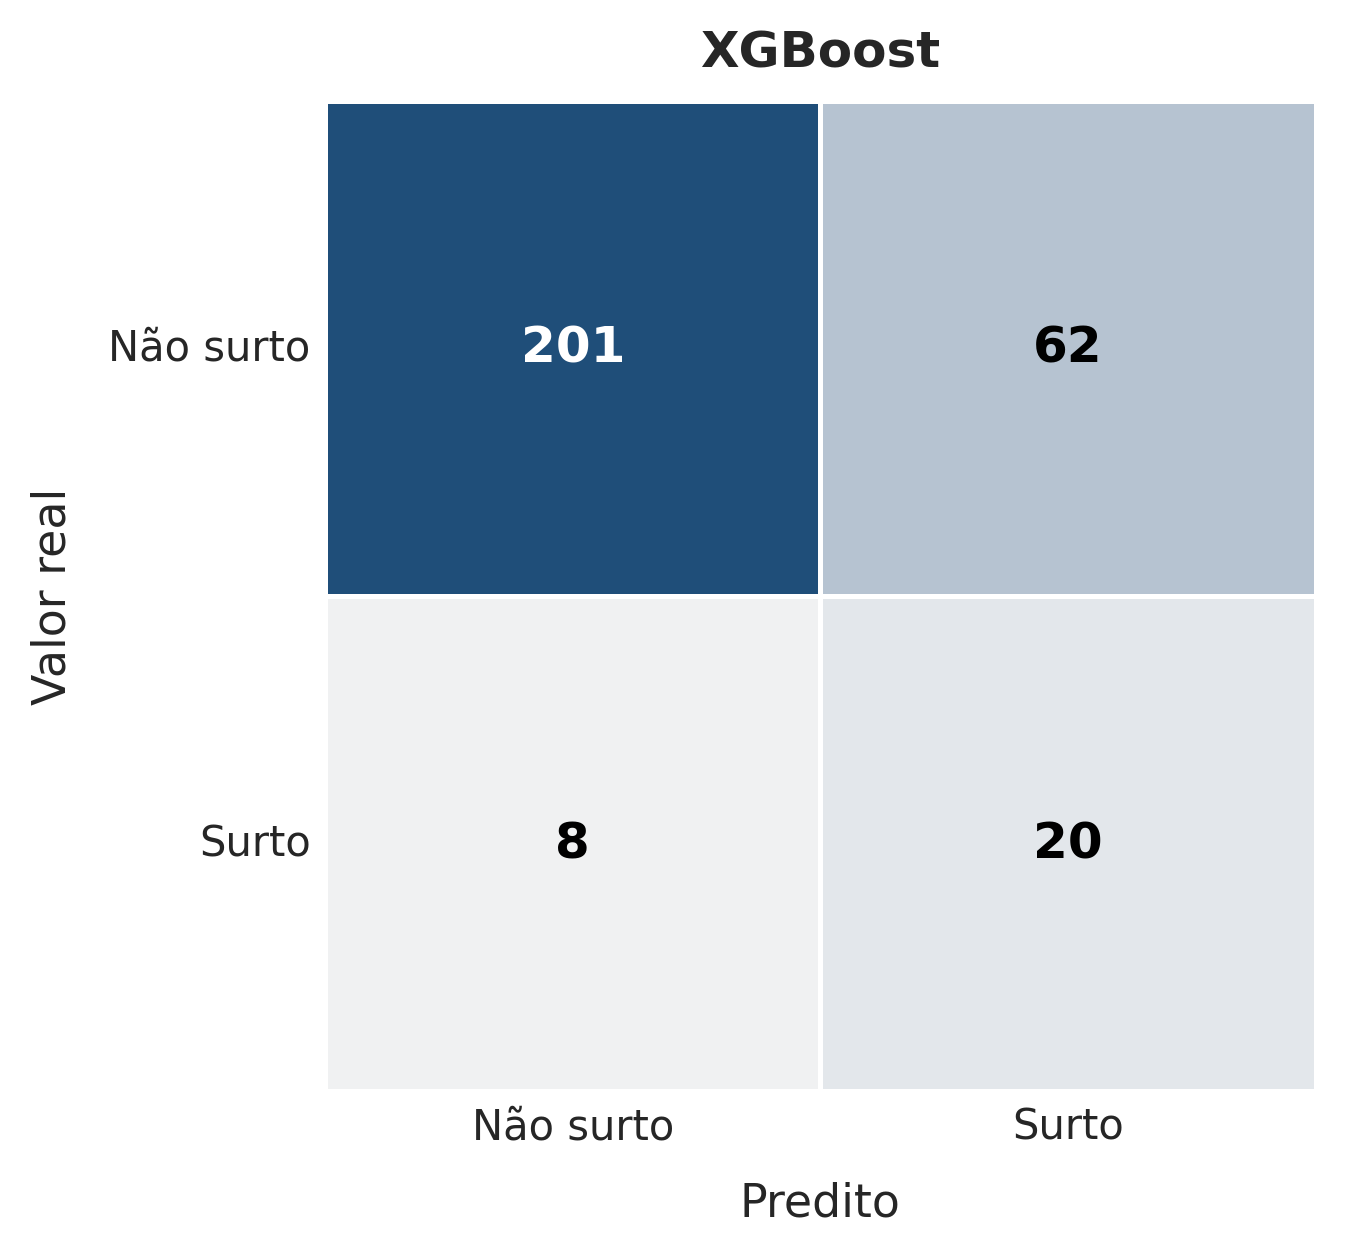
\includegraphics[width=\textwidth]{figs/confusion_clean/xgb_clean.png}
\caption{XGBoost}
\label{fig:confusao-xgb}
\end{subfigure}
\hfill
\begin{subfigure}[t]{0.47\textwidth}
\centering
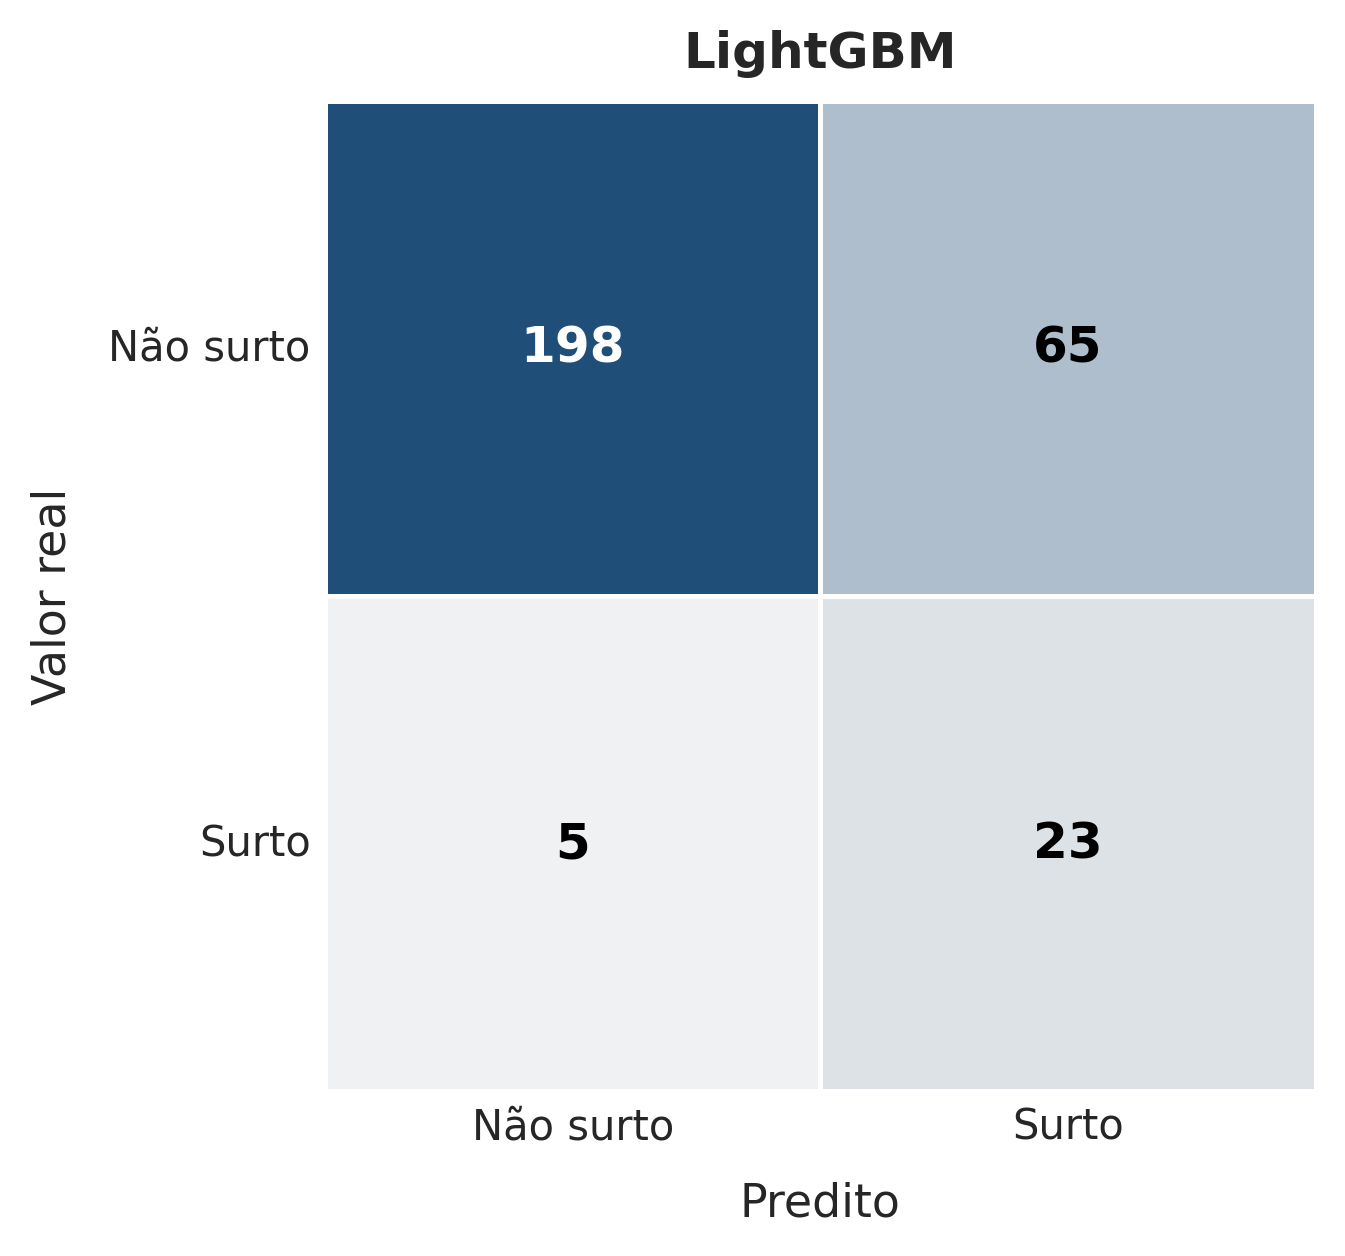
\includegraphics[width=\textwidth]{figs/confusion_clean/lgbm_clean.png}
\caption{LightGBM}
\label{fig:confusao-lgbm}
\end{subfigure}

\vspace{0.6cm}

\begin{subfigure}[t]{0.47\textwidth}
\centering
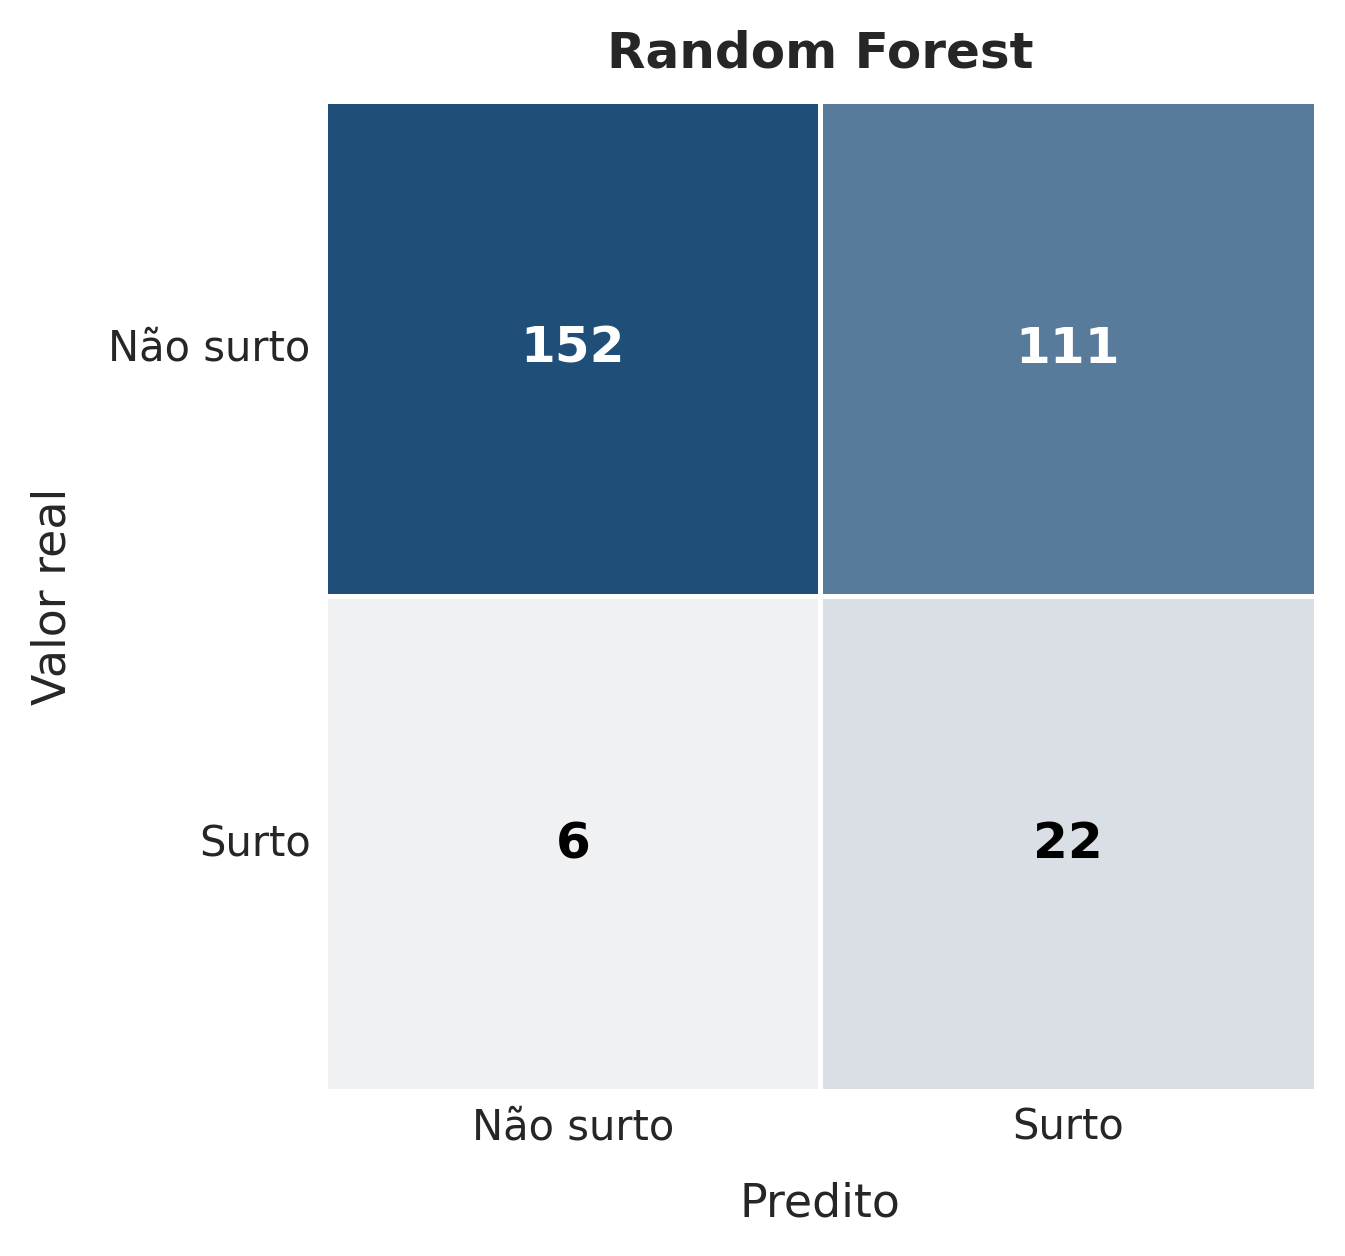
\includegraphics[width=\textwidth]{figs/confusion_clean/rf_clean.png}
\caption{Random Forest}
\label{fig:confusao-rf}
\end{subfigure}
\artigofonte{elabora\c{c}\~ao pr\'opria.}
\end{figure}

A Figura \ref{fig:confusoes} mostra que o ganho do LightGBM n\~ao decorre apenas de maior sensibilidade, mas de melhor equil\'ibrio entre recupera\c{c}\~ao de surtos e estabilidade probabil\'istica. Esse padr\~ao \'e compat\'ivel com os valores de AUC-PR e \textit{Brier Score}, que favorecem o LightGBM em rela\c{c}\~ao aos demais modelos.

Do ponto de vista interpretativo, isso explicita uma diferen\c{c}a importante frente a compara\c{c}\~oes mais gen\'ericas de algoritmos: neste trabalho, a utilidade do modelo \'e analisada tamb\'em pelo custo operacional de falsos alertas. Esse enquadramento aproxima a avalia\c{c}\~ao do cen\'ario concreto da vigil\^ancia epidemiol\'ogica.

\eventsubsection{An\'alise complementar}

A an\'alise de import\^ancia de atributos mostrou converg\^encia parcial entre os modelos. O atributo \texttt{casos\_novos\_malaria\_trend} apareceu como principal preditor nos tr\^es algoritmos, indicando que a din\^amica recente da s\'erie epidemiol\'ogica concentra a maior parte do sinal para discrimina\c{c}\~ao de surtos. Nos modelos de \textit{boosting}, vari\'aveis clim\'aticas e de intera\c{c}\~ao tamb\'em tiveram participa\c{c}\~ao relevante, o que sugere complementaridade entre hist\'orico epidemiol\'ogico e sazonalidade ambiental.

\begin{table}[H]
\centering
\caption{Principais atributos para classifica\c{c}\~ao de surto por modelo.}
\label{tab:atributos}
\tabelafonte
\begin{tabular}{lll}
\toprule
Posi\c{c}\~ao & XGBoost & LightGBM \\
\midrule
1 & \texttt{casos\_novos\_malaria\_trend} & \texttt{casos\_novos\_malaria\_trend} \\
2 & \texttt{dias\_com\_chuva\_lag3} & \texttt{temp\_x\_casos\_ma3} \\
3 & \texttt{chuva\_total\_mes\_ma3} & \texttt{casos\_novos\_malaria\_ma6} \\
4 & \texttt{umid\_media\_mes\_ma3} & \texttt{temp\_max\_media\_mes\_ma6} \\
5 & \texttt{temp\_media\_mes} & \texttt{casos\_novos\_malaria\_ma3} \\
\bottomrule
\end{tabular}
\artigofonte{elabora\c{c}\~ao pr\'opria com base nos relat\'orios de import\^ancia de atributos.}
\end{table}

Os testes de abla\c{c}\~ao e de robustez temporal refor\c{c}aram essa interpreta\c{c}\~ao. O uso isolado de vari\'aveis clim\'aticas gerou desempenho fraco, enquanto o bloco epidemiol\'ogico preservou parte relevante da capacidade discriminativa. Quando as duas fontes de informa\c{c}\~ao foram combinadas, o desempenho melhorou de modo consistente. Em termos temporais, o LightGBM manteve ordena\c{c}\~ao probabil\'istica \'util mesmo quando avaliado por ano, embora com oscila\c{c}\~ao do F1 conforme o regime epidemiol\'ogico.

Esse resultado refor\c{c}a outra contribui\c{c}\~ao do estudo: mostrar que a superioridade do modelo n\~ao depende exclusivamente de um recorte agregado de teste, mas se preserva de forma razo\'avel quando o problema \'e reobservado sob varia\c{c}\~ao anual e sob redefini\c{c}\~oes operacionais do alvo.

\begin{table}[H]
\centering
\caption{Resumo de abla\c{c}\~ao, robustez temporal e sensibilidade do alvo.}
\label{tab:ablation}
\tabelafonte
\begin{tabular}{lcccc}
\toprule
Cen\'ario & ROC-AUC & PR-AUC & F1 & Brier \\
\midrule
Completo & 0,864 & 0,536 & 0,489 & 0,067 \\
Sem intera\c{c}\~oes & 0,872 & 0,568 & 0,508 & 0,061 \\
Epidemiol\'ogico apenas & 0,804 & 0,352 & 0,491 & 0,091 \\
Clim\'atico apenas & 0,563 & 0,210 & 0,205 & 0,108 \\
Clima + epidemiologia & 0,873 & 0,569 & 0,508 & 0,060 \\
\midrule
Robustez 2023 & 0,714 & 0,469 & 0,444 & 0,069 \\
Robustez 2024 & 0,862 & 0,630 & 0,375 & 0,054 \\
Robustez 2025 & 0,878 & 0,415 & 0,218 & 0,080 \\
\midrule
Quantil 0,85 & 0,764 & 0,339 & -- & 0,115 \\
Quantil 0,90 & 0,704 & 0,380 & -- & 0,099 \\
Quantil 0,95 & 0,767 & 0,281 & -- & 0,053 \\
\bottomrule
\end{tabular}
\artigofonte{elabora\c{c}\~ao pr\'opria a partir dos relat\'orios de abla\c{c}\~ao, robustez temporal e valida\c{c}\~ao adicional.}
\end{table}

Os valores da Tabela \ref{tab:ablation} indicam que o modelo n\~ao depende exclusivamente das vari\'aveis clim\'aticas, mas tamb\'em n\~ao se sustenta apenas sobre uma l\'ogica ambiental simplificada. A melhor resposta emerge da combina\c{c}\~ao entre clima e hist\'orico recente de casos. Al\'em disso, a sensibilidade a diferentes quantis de defini\c{c}\~ao de surto mostrou queda moderada, e n\~ao colapso, o que \'e um sinal importante de estabilidade conceitual do pipeline.

Em termos interpretativos, os achados sustentam a ado\c{c}\~ao de modelos de \textit{boosting} em sistemas de alerta epidemiol\'ogico para mal\'aria no Amazonas, especialmente quando o objetivo \'e priorizar eventos raros com depend\^encia temporal. Ainda assim, alguns limites precisam ser considerados. O estudo permanece restrito ao Amazonas, a defini\c{c}\~ao de surto foi operacionalizada por quantil municipal e o n\'umero absoluto de eventos positivos no teste ainda \'e relativamente pequeno. Portanto, embora os resultados sejam consistentes, a generaliza\c{c}\~ao para outros contextos exige valida\c{c}\~ao adicional.

Essa delimita\c{c}\~ao tamb\'em ajuda a posicionar corretamente o alcance do artigo. A contribui\c{c}\~ao aqui produzida \'e uma evid\^encia aplicada, metodologicamente rigorosa e contextualizada para a Amaz\^onia, e n\~ao uma afirma\c{c}\~ao universal sobre superioridade de um algoritmo em qualquer cen\'ario epidemiol\'ogico.

Do ponto de vista de governan\c{c}a e reprodutibilidade, a arquitetura do pipeline foi mantida modular, com separa\c{c}\~ao clara entre pr\'e-processamento, treinamento e gera\c{c}\~ao de relat\'orios. Essa organiza\c{c}\~ao facilita auditoria, reexecu\c{c}\~ao e atualiza\c{c}\~ao por novas janelas temporais. O fluxo tamb\'em tolera execu\c{c}\~ao heterog\^enea, com acelera\c{c}\~ao por GPU quando dispon\'ivel e alternativa est\'avel em CPU, sem alterar o protocolo metodol\'ogico. Em cen\'arios de uso real, recomenda-se complementar o modelo com monitoramento de deriva, recalibra\c{c}\~ao de limiares e rastreabilidade de vers\~oes, em sintonia com recomenda\c{c}\~oes de governan\c{c}a para IA em sa\'ude \cite{world2024ethics}.

\eventsection{CONSIDERA\c{C}\~OES FINAIS}

O estudo comparou algoritmos de \textit{bagging} e \textit{boosting} para detec\c{c}\~ao de surtos de mal\'aria no estado do Amazonas com base em um protocolo temporal rigoroso. Os resultados indicaram desempenho superior do LightGBM em rela\c{c}\~ao ao XGBoost e ao Random Forest, tanto em capacidade discriminativa quanto em qualidade probabil\'istica. Esse achado sugere que modelos de \textit{boosting} s\~ao mais adequados para apoiar sistemas de alerta em contextos epidemiol\'ogicos com baixa preval\^encia de surtos.

Como implica\c{c}\~ao pr\'atica, a aplica\c{c}\~ao desses modelos pode contribuir para orientar monitoramento preventivo, prioriza\c{c}\~ao territorial e revis\~ao de limiares de risco em rotinas de vigil\^ancia. No entanto, o uso operacional deve permanecer vinculado \`a avalia\c{c}\~ao t\'ecnica das equipes de sa\'ude, com monitoramento cont\'inuo de desempenho, recalibra\c{c}\~ao peri\'odica e transpar\^encia sobre os crit\'erios de decis\~ao.

Como trabalhos futuros, recomenda-se ampliar a valida\c{c}\~ao para diferentes recortes geogr\'aficos, explorar calibra\c{c}\~ao probabil\'istica formal e comparar o ajuste por peso de classe com t\'ecnicas de reamostragem e abordagens custo-sens\'iveis, como SMOTE e aprendizado custo-sens\'ivel \cite{chawla2002smote,elkan2001foundations}. Tamb\'em s\~ao relevantes estudos com m\'ultiplos anos, deriva de atributos, monitoramento de preval\^encia e estabilidade da taxa de alertas por munic\'ipio. Essas extens\~oes podem fortalecer a robustez metodol\'ogica e a aplicabilidade do sistema em outros cen\'arios amaz\^onicos.


\postextual
\bibliography{referencias}

\end{document}
